\documentclass[10pt,a4paper]{article}
\usepackage[utf8x]{inputenc}
\usepackage{ucs}
\usepackage{amsmath}
\usepackage{amsfonts}
\usepackage{amssymb}
\usepackage{graphicx}
\usepackage{moreverb} 
\usepackage{hyperref}
\usepackage{colortbl}
\pagestyle{headings}

\begin{document}
\renewcommand{\contentsname}{Indice} 
\renewcommand\listfigurename{Lista de Figuras}
\renewcommand\listtablename{Lista de Tablas}
\newcommand\bibname{Bibliografía}
\renewcommand{\refname}{Bibliografía}
\renewcommand\indexname{Indice alfabético}
\renewcommand\figurename{Figura}
\renewcommand\tablename{Tabla}
\renewcommand\partname{Parte}
\newcommand\chaptername{Capítulo}
\renewcommand\appendixname{Apéndice}
\renewcommand\abstractname{Resumen}

\title{Sexta semana de trabajo [05 - 09 de Mayo]}
\author{Milton Inostroza Aguilera}
\date{12 Mayo de 2008}
\clearpage
\maketitle

\begin{abstract}

Se modifica borrador de protocolo para mejor adpatación entre pyTOD y TOD:
\begin{itemize}
\item parentId en el registro de probe cambia de posición.
\item typeId se agrega como antecesor de cualquier valor que se envíe a la base de datos de TOD.
\end{itemize}
\\
Se ha logrado obtener los primeros resultados de la depuración a un script escrito en Python, pero aún existen problemas para ver los registros desde el lado de TOD.  Se detectó timestamp's que apuntaban ciclicamente a si mismos.


\end{abstract}
\newpage
\tableofcontents
\newpage
\listoffigures
\newpage
\listoftables
\newpage
\section{Desarrollo}

Se hicieron pequeños cambios al borrador del protocolo de comunicación específicamente en el momento que se envía un valor desde pyTOD hacia TOD.  Se agregó un identificador de tipo de datos para manipularlo de forma correcta, tanto para envíarlo como para recibirlo.\\

El socket servidor ya está completamente implementado en el lado Java y se comunica de forma satisfactoria con su cliente en el lado Python.\\

Empieza a ser necesaria la modificación de la máquina virtual de Python o la creación de un tipo de datos nativo especial que permita implementar el identificador único para ver como se comporta pyTOD con este tipo de objetos.



\section{Protocolo de comunicación - Draft}

Se muestran las tablas bases para el registro de los objetos y para el envío de eventos:

\subsection{Identificadores bases}

La siguiente tabla muestra que cada suceso tiene un identificador en el sistema de capturación de huella.
\begin{table}[!h]
\begin{center}
\begin{tabular}{|l | c |}
\hline
Suceso & Identificador\\
\hline
Registro & 0\\
\hline
Llamada & 1\\
\hline
Retorno & 2\\
\hline
Asignacion & 3\\
\hline
\end{tabular}
\caption{Identificadores de sucesos} 
\end{center}
\end{table}

La siguiente tabla muestra que cada objeto tiene un identificador en el sistema de capturación de huella.
\begin{table}[!h]
\begin{center}
\begin{tabular}{|l | c |}
\hline
Id Objeto & Identificador\\
\hline
Clase & 0\\
\hline
método & 1\\
\hline
Atributo & 2\\
\hline
Funcion & 3\\
\hline
Variable local & 4\\
\hline
Probe & 5\\
\hline
Thread & 6\\
\hline
\end{tabular}
\caption{Identificadores de objetos} 
\end{center}
\end{table}
\\
\pagebreak

La siguiente tabla muestra que cada tipo de datos un identificador en el sistema de capturación de huella.
\begin{table}[!h]
\begin{center}
\begin{tabular}{|l | c |}
\hline
Type & Identificador\\
\hline
int & 0\\
\hline
str & 1\\
\hline
float & 2\\
\hline
long & 3\\
\hline
bool & 4\\
\hline
other & 5\\
\hline
\end{tabular}
\caption{Identificadores de tipo de datos} 
\end{center}
\end{table}

\subsection{Registro de objetos}

A continuación se muestra el formato que tienen el registro de los diferentes objetos dentro del capturador de huellas:\\

Se describe el registro del objeto función:\\

\begin{table}[!h]
\begin{center}
\begin{tabular}{| c | c | c | c | c | c | c |}
\hline
eventId & objectId & Id & name & argsN & \{argName_{i} & argId_{i}\}\\
\hline
int & int & int & str & int & str & int \\
\hline
\end{tabular}
\caption{Registro del objeto función} 
\end{center}
\end{table}


Se describe el registro del objeto variable local:\\

\begin{table}[!h]
\begin{center}
\begin{tabular}{| c | c | c | c | c |}
\hline
eventId & objectId & Id & parentId & name\\
\hline
int & int & int & int & str\\
\hline
\end{tabular}
\caption{Registro del objeto variable local} 
\end{center}
\end{table}


Se describe el registro del objeto clase:\\

\begin{table}[!h]
\begin{center}
\begin{tabular}{| c | c | c | c | c |}
\hline
eventId & objectId & Id & name & classBases\\
\hline
int & int & int & str & --\footnotemark[1]\\
\hline
\end{tabular}
\caption{Registro del objeto clase} 
\end{center}
\end{table}


\footnotetext[1]{Aún no se toma decisión para poder registrar las super clases que pueda tener la clase registrada.}
\newpage
Se describe el registro del objeto método:\\

\begin{table}[!h]
\begin{center}
\begin{tabular}{| c | c | c | c | c | c | c | c |}
\hline
eventId & objectId & Id & classId & name & argsN & \{argName_{i} & argId_{i}\}\\
\hline
int & int & int & int & str & int & str & int \\
\hline
\end{tabular}
\caption{Registro del objeto método} 
\end{center}
\end{table}


Se describe el registro del objeto atributo:\\

\begin{table}[!h]
\begin{center}
\begin{tabular}{| c | c | c | c | c |}
\hline
eventId & objectId & Id & parentId & name\\
\hline
int & int & int & int & str\\
\hline
\end{tabular}
\caption{Registro del objeto atributo} 
\end{center}
\end{table}


Se describe el registro del objeto thread: \\

\begin{table}[!h]
\begin{center}
\begin{tabular}{| c | c | c | c |}
\hline
eventId & objectId & Id & sysId\\
\hline
int & int & int & int\\
\hline
\end{tabular}
\caption{Registro del objeto thread} 
\end{center}
\end{table}


Se describe el registro del objeto probe: \\

\begin{table}[!h]
\begin{center}
\begin{tabular}{| c | c | c | c | c |}
\hline
eventId & objectId & Id & parentId & currentLasti \\
\hline
int & int & int & int & int\\
\hline
\end{tabular}
\caption{Registro del objeto probe} 
\end{center}
\end{table}

\newpage
\subsection{Llamada de objetos}

A continuación se muestra el formato que tienen las llamadas de los objetos función y método dentro del capturador de huellas:\\

Se describe la llamada al objeto función:\\

\begin{table}[!h]
\begin{center}
\begin{tabular}{| c | c | c | c | c | c | c |}
\hline
eventId & objectId & Id & parentId & argsN & typeId_{i} & argValue_{i}\\
\hline
int & int & int & int & int & --\footnotemark[1]\\
\hline
\end{tabular}
\caption{Llamada al objeto función} 
\end{center}
\end{table}

Se describe la llamada al objeto método:\\

\begin{table}[!h]
\begin{center}
\begin{tabular}{| c | c | c | c | c | c | c | c |}
\hline
eventId & objectId & Id & parentId & classId & argsN & typeId_{i} & argValue_{i}\\
\hline
int & int & int & int & int & int & --\footnotemark[1]\\
\hline
\end{tabular}
\caption{Llamada al objeto método} 
\end{center}
\end{table}

Es importante señalar que todas estas llamadas estan acompañadas de los siguientes datos que se describen a continuación:\\

\begin{table}[!h]
\begin{center}
\begin{tabular}{| c | c | c | c | c |}
\hline
probeId & parentTimeStampFrame & depth & currentTimeStamp & threadId\\
\hline
int & double & int & double & int \\
\hline
\end{tabular}
\caption{Coordenadas} 
\end{center}
\end{table}


\footnotetext[1]{Aún no se toma decisión para poder almacenar los valores de objetos primitivos de Python como son: listas, tuplas, diccionarios, enumeraciones.}
\newpage

\subsection{Asignación - Modificación de objetos}
A continuación se muestra el formato que tienen las asignaciones | modificaciones de los objetos variable local y atributo dentro del capturador de huellas:\\

Se describe la asignación - modificacion al objeto variable local:\\

\begin{table}[!h]
\begin{center}
\begin{tabular}{| c | c | c | c | c | c |}
\hline
eventId & objectId & Id & parentId & typeId & value\\
\hline
int & int & int & int & --\footnotemark[1]\\
\hline
\end{tabular}
\caption{Registro del objeto variable local} 
\end{center}
\end{table}

Se describe la asignación - modificación al objeto atributo:\\

\begin{table}[!h]
\begin{center}
\begin{tabular}{| c | c | c | c | c | c |}
\hline
eventId & objectId & Id & parentId & typeId & value\\
\hline
int & int & int & int & --\footnotemark[1]\\
\hline
\end{tabular}
\caption{Registro del objeto atributo} 
\end{center}
\end{table}

Es importante señalar que todas estas asignaciones - modificaciones estan acompañadas de los siguientes datos que se describen a continuación:\\

\begin{table}[!h]
\begin{center}
\begin{tabular}{| c | c | c | c | c |}
\hline
probeId & parentTimeStampFrame & depth & currentTimeStamp & threadId\\
\hline
int & double & int & double & int \\
\hline
\end{tabular}
\caption{Coordenadas} 
\end{center}
\end{table}

\subsection{Return}

A continuación se muestra el formato que tiene el return dentro del capturador de huellas:\\

Se describe return:\\

\begin{table}[!h]
\begin{center}
\begin{tabular}{| c | c | c | c | c |}
\hline
eventId & typeId & value & probeId & hasThrown \\
\hline
int & --\footnotemark[1] & int & bool\\
\hline
\end{tabular}
\caption{Registro de return} 
\end{center}
\end{table}

\footnotetext[1]{Aún no se toma decisión para poder almacenar los valores de objetos primitivos de Python como son: listas, tuplas, diccionarios, enumeraciones.}

\newpage
\section{Primeras depuraciones}

Se ha logrado realizar las primeras depuraciones, pero aún no son lo completas que deseamos.  Se está trabajando en encontrar las incompatibilidades que se están generando entre el modelo actual de huella de TOD con el modelo propuesto de huella de pyTOD.  Aún teniendo ciertos problemas y bugs es posible ver algunas opciones gráficas ya disponibles.\\

Se ha depurado parcialmente el siguiente trozo de código:\\

\begin{verbatim}
class clase1(Descriptor):
    
    def __init__(self, y):
        self.x = 1
        self.c = 2
        self.z = 3
        return
    
    def metodo(self, h, i, j, k):
        self.casa = 1
        k = i + j
        return
\end{verbatim}

TOD, nos muestra la siguiente información:\\

\begin{figure}[hpb]
	\centering
	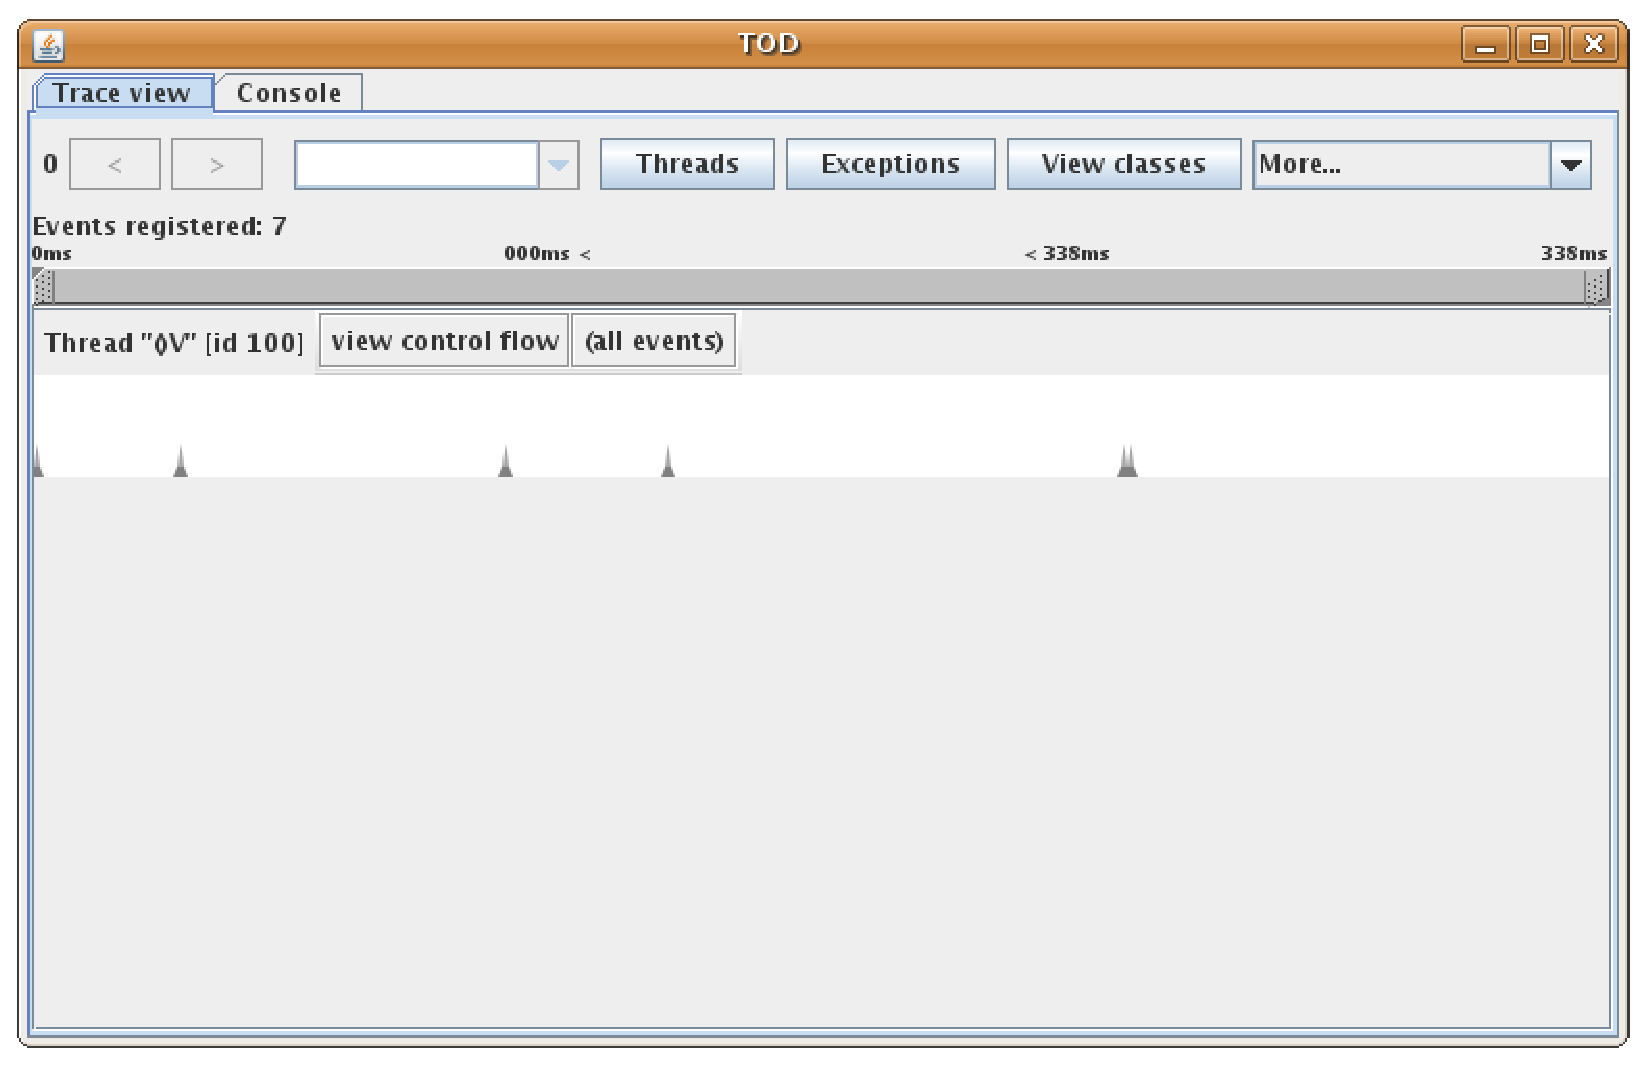
\includegraphics[scale=0.5]{images/TOD-1.eps}
	\caption{Pantalla principal de TOD}
\end{figure}

\begin{figure}[hpb]
	\centering
	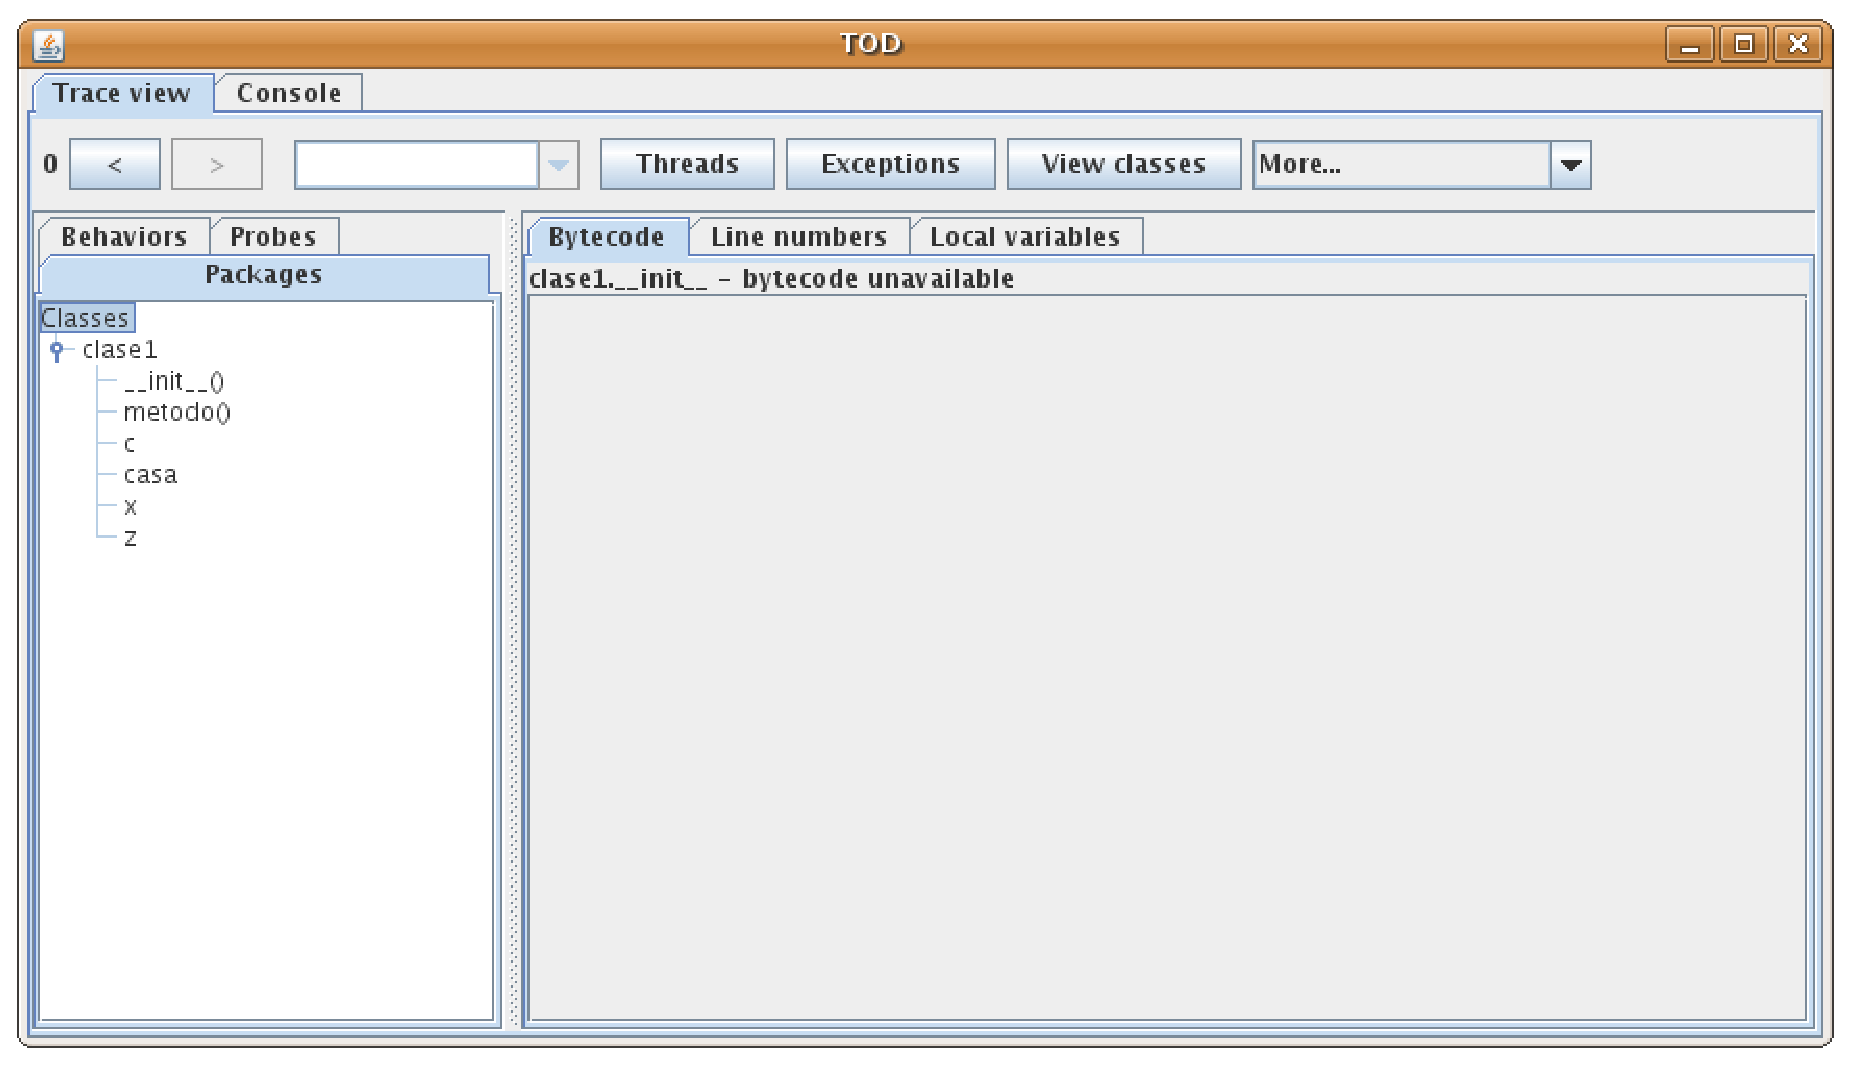
\includegraphics[scale=0.5]{images/TOD-2.eps}
	\caption{Clases son sus métodos y atributos}
\end{figure}

\begin{figure}[hpb]
	\centering
	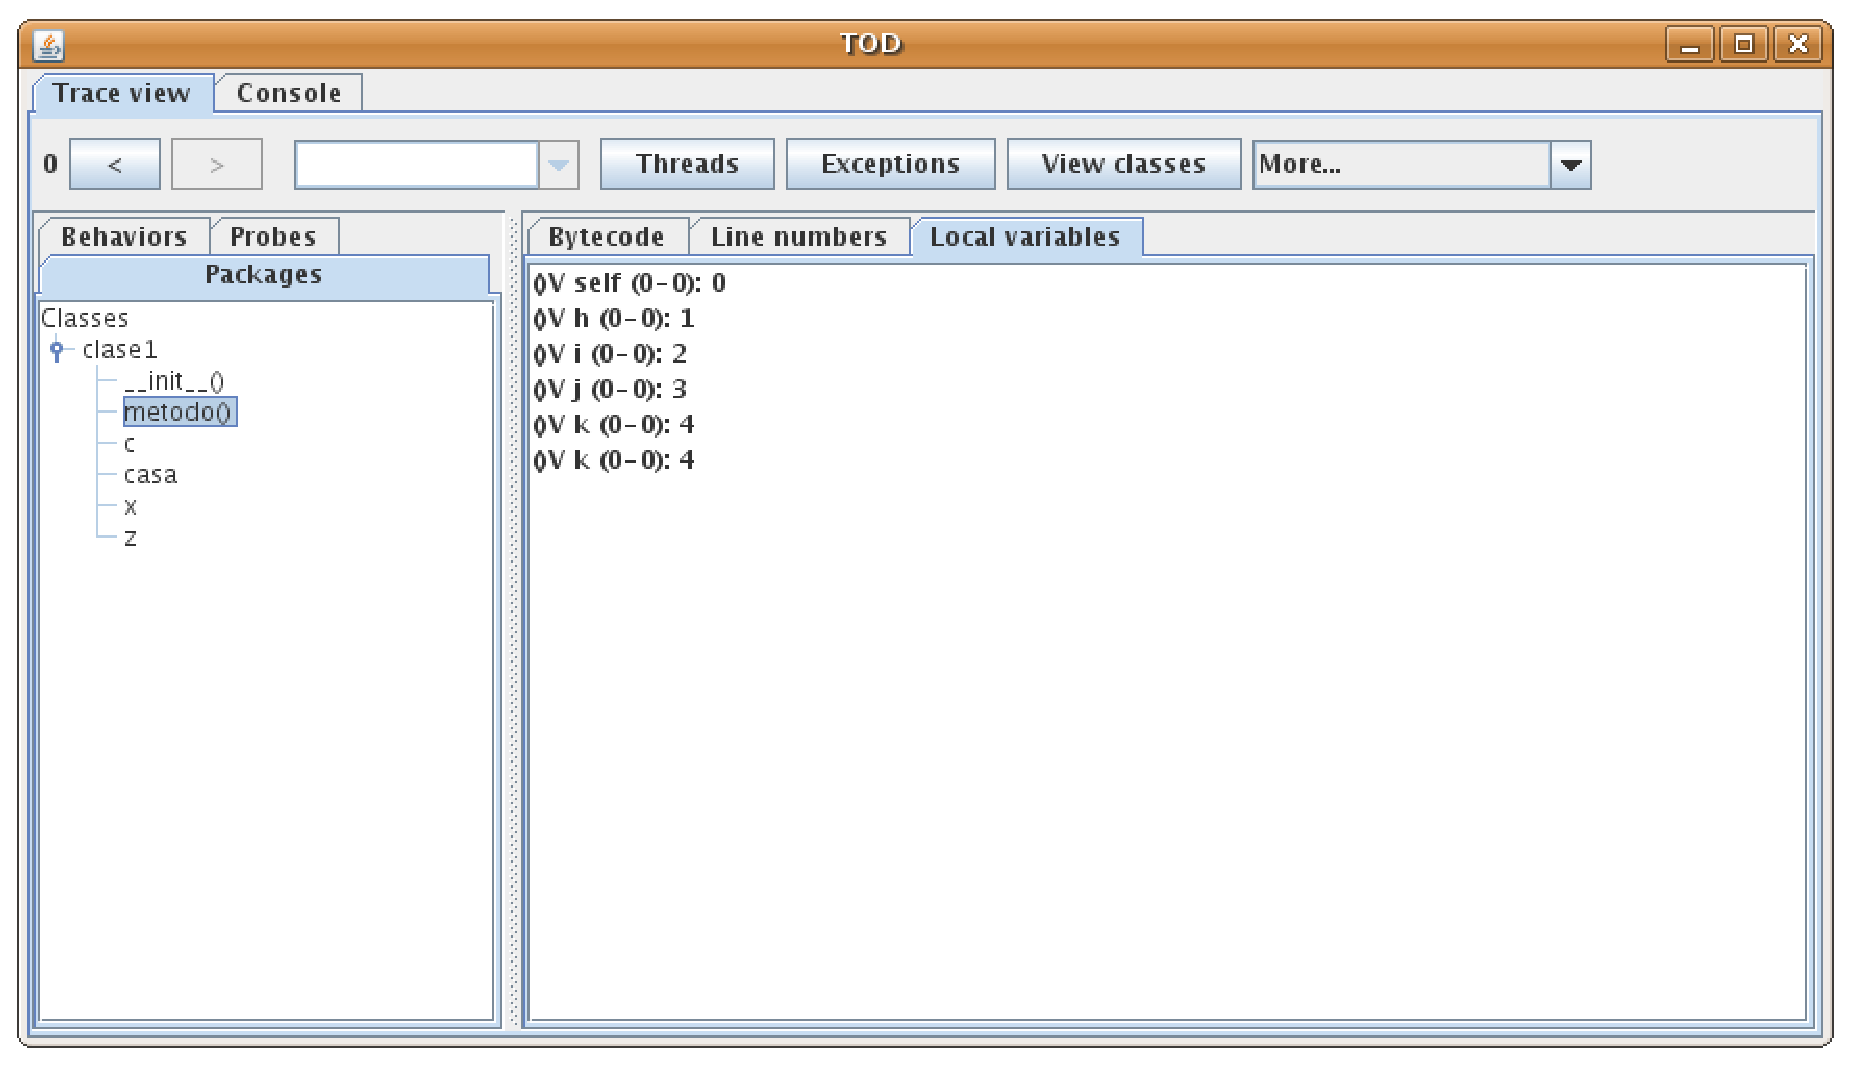
\includegraphics[scale=0.5]{images/TOD-4.eps}
	\caption{Métodos con sus variables locales}
\end{figure}

\newpage
\begin{figure}[hpb]
	\centering
	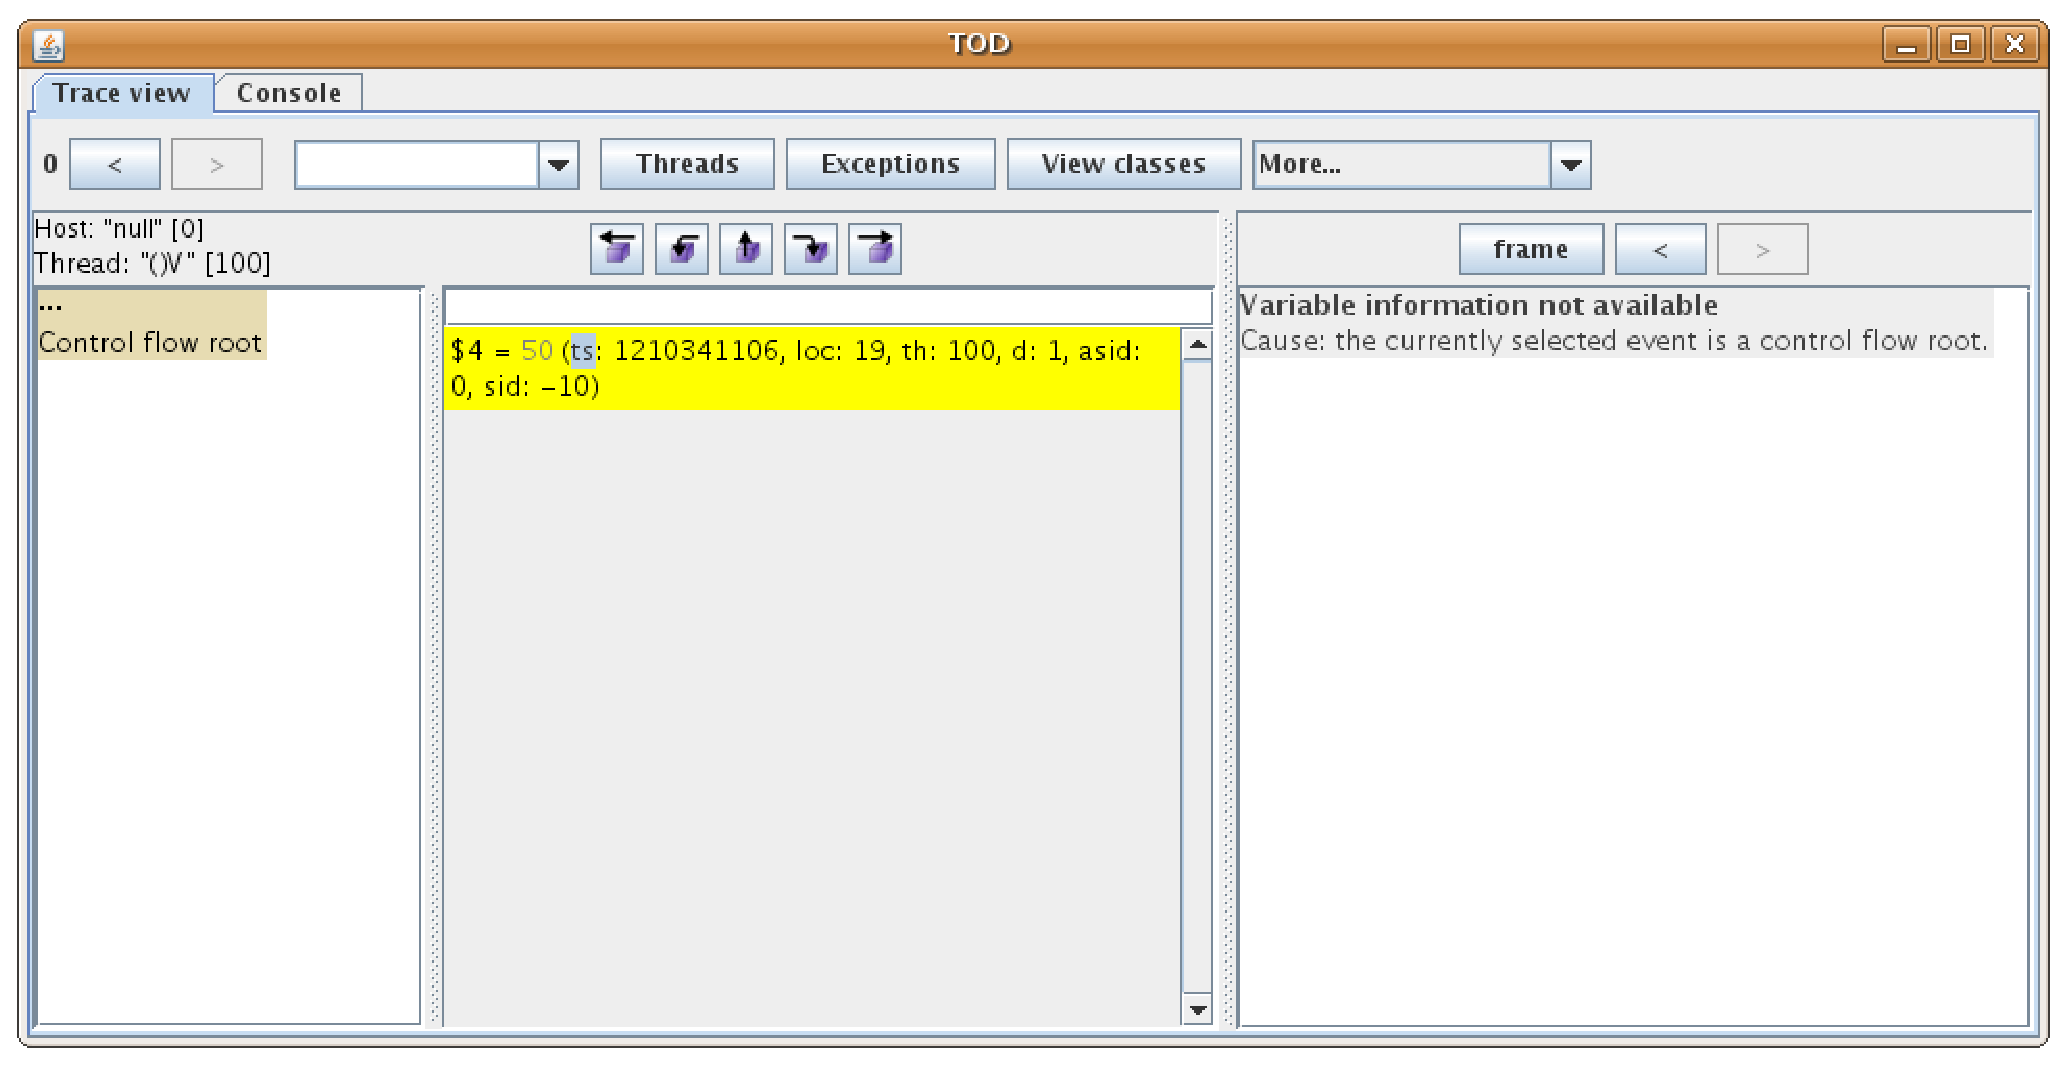
\includegraphics[scale=0.4]{images/TOD-5.eps}
	\caption{Vista de los eventos ocurridos}
\end{figure}

Lamentablemente en esta última pantalla se debieran ver siete eventos y sólo se ve uno.  Esto es parte del problema descrito anteriormente.

\newpage
\begin{thebibliography}{2}
\bibitem{id} \url{http://docs.python.org/lib/built-in-funcs.html}
\bibitem{howto} \url{http://docs.python.org/ext/ext.html}
\end{thebibliography}
\end{document}
